% !TeX encoding = utf8
\documentclass[german,aspectratio=169]{beamer}
\usepackage{beamerthemeHM} 
\usepackage{graphicx}

% These are some nice colors that fit well together
\definecolor{midnightblue}{RGB}{10,10,44}
\definecolor{navyblue}{RGB}{0,0,120}
\definecolor{crimson}{RGB}{220,20,60}
\definecolor{mydarkgray}{RGB}{33,33,33}
\definecolor{myalgColor}{RGB}{99,99,99}
\definecolor{mygreen}{RGB}{85,168,104}
\definecolor{myorange}{RGB}{221,132,82}
\definecolor{myblue2}{rgb}{0.12156862745098039, 0.4666666666666667, 0.7058823529411765}
\definecolor{myblue3}{rgb}{0.2980392156862745, 0.4470588235294118, 0.6901960784313725}
\definecolor{myblue4}{rgb}{0.2823529411764706, 0.47058823529411764, 0.8156862745098039}
\definecolor{mybluebright}{rgb}{0.00784313725490196, 0.24313725490196078, 1.0}
\definecolor{myred}{RGB}{196,78,82}
\definecolor{mydarkgray}{RGB}{90,90,90}
\definecolor{mygray}{RGB}{179,179,179}
\definecolor{myviolet}{RGB}{129,114,178}
\definecolor{myblue}{RGB}{76,114,202}
\xdefinecolor{mybg}{rgb}{0.7419607843137255, 0.9027297193387159, 0.868958093041138}
\xdefinecolor{myRed}{rgb}{0.7686274509803922, 0.3058823529411765, 0.3215686274509804}
\xdefinecolor{prevColor}{rgb}{0.39215686274509803, 0.7098039215686275, 0.803921568627451}
\xdefinecolor{mylightblue}{rgb}{0.8584083044982699, 0.9134486735870818, 0.9645674740484429}

\definecolor{mybrightblue}{rgb}{0.00784313725490196, 0.24313725490196078, 1.0}
\definecolor{mybrightred}{rgb}{0.9098039215686274, 0.0, 0.043137254901960784}

\xdefinecolor{myalgColor}{rgb}{0.7686274509803922, 0.3058823529411765, 0.3215686274509804}

% hm colors
\xdefinecolor{hmred}{RGB}{252, 85, 85}

%
\xdefinecolor{colordefinition}{RGB}{0, 123, 255}
\xdefinecolor{colorexample}{RGB}{200, 200, 200}

% listing colors
\definecolor{codegreen}{rgb}{0,0.6,0}
\definecolor{codegray}{rgb}{0.5,0.5,0.5}
\definecolor{codepurple}{rgb}{0.58,0,0.82}
\definecolor{backcolour}{rgb}{0.95,0.95,0.92}

\definecolor{halfgray}{gray}{0.55}
\definecolor{ipython_frame}{RGB}{207, 207, 207}
\definecolor{ipython_bg}{RGB}{247, 247, 247}
\definecolor{ipython_red}{RGB}{186, 33, 33}
\definecolor{ipython_green}{RGB}{0, 128, 0}
\definecolor{ipython_cyan}{RGB}{64, 128, 128}
\definecolor{ipython_purple}{RGB}{170, 34, 255}

%packages%
\usepackage{savesym}
\usepackage{longtable}
\usepackage{listings}
\usepackage{placeins}
\usepackage{media9}
\usepackage{appendixnumberbeamer}
%\usepackage{multimedia}
%\usepackage{animate}
\usepackage[font=itshape,noorphans=true]{quoting}

%font
\usepackage{amsmath,amsfonts,amsthm,amssymb,mathtools,stmaryrd,xpatch}
\usepackage[T1]{fontenc}
\usepackage{marvosym} 
\usepackage{libertine}
\usepackage[libertine]{newtxmath}

% german symbols
\usepackage[utf8]{inputenc}

\usepackage{array}
\usepackage{makecell}
\usepackage{graphicx}
\usepackage{color}
\usepackage{emptypage}
\usepackage[toc,page]{appendix}
\usepackage{listings}

%\usepackage[format=plain, skip=5pt, labelfont=bf]{caption}
\usepackage{subfigure}
%\usepackage[labelfont=normalfont]{subcaption}
%\usepackage[ngerman,english]{babel}
\usepackage[ngerman]{babel}
%\usepackage{polyglossia}%german beamer commands
\usepackage{tikz}
\usetikzlibrary{%
	positioning,calc,trees,positioning,automata,arrows,chains,shapes.geometric,%
	decorations.pathreplacing,decorations.pathmorphing,shapes,%
	matrix,shapes.symbols%
}%
\let\openbox\undefined
\usepackage[vlined,linesnumbered,resetcount]{algorithm2e}
\usepackage[numbers]{natbib}
\usepackage{bussproofs}
\usepackage{stackengine}
\usepackage{enumitem}
\usepackage{framed}
\usepackage{url}
\urlstyle{same}
\usepackage[capitalise]{cleveref}
\usepackage{hyperref}



% Zahlen, Mengen, Intervalle, Addieren, Multiplizieren, Subtrahieren, Dividieren
\title{\huge Computational Thinking}
\subtitle{Algorithmisches Denken mithilfe von Jupyter-Notebooks}
\author{Prof. Martin Hobelsberger \\ \href{mailto:zoennchen.benedikt@hm.edu}{Dr. Benedikt Zönnchen}}
\date{19. Mai 2022}
\institute{	
\includegraphics[height=15pt]{./figs/Hochschule_Muenchen_Logo}}
\begin{document}

\begin{frame}
 \titlepage
\end{frame}

%\begin{frame}
%	\frametitle{}
%	Algorithmisches Denken im Alltag:
%	\begin{quoting}
%		``Plans with people that pass the entire cognitive load to them rarely materialize.'' -- Algorithms to Live By
%	\end{quoting}
%\end{frame}

\begin{frame}
	\frametitle{Herausforderung}
	Vielfältige interdisziplinäre CSPlus / PlusCS Studiengänge der Hochschule München:
	\begin{enumerate}[label=$\bullet$]
		\item Digital Engineering
		\item Informatik und Design
		\item Geodata Science
		\item Data Science \& Scientific Computing
		\item $\ldots$ (in der Zukunft)
	\end{enumerate}
	$\Rightarrow$ Erhöhte Heterogenität der Studierenden
\end{frame}

\begin{frame}
	\frametitle{Herausforderung}
	Studierenden jener Studiengänge soll es möglich sein
	\begin{quoting}
		\glqq\textbf{Problemstellungen} zu \textbf{identifizieren}, \textbf{abstrakt} zu \textbf{modellieren}, sie dabei in \textbf{Teilprobleme} zu \textbf{zerlegen}, \textbf{Lösungsstrategien} zu \textbf{entwerfen} und auszuarbeiten und diese \textbf{formalisiert} \textbf{darzustellen}, sodass sie von einem Menschen (oder auch einem Computer) verstanden und ausgeführt werden können.\grqq
	\end{quoting}
	Kurz gesagt: Studierende sollen \textbf{Computational Thinking (CT)} beherrschen.
\end{frame}

\begin{frame}
	\frametitle{Was verstehen wir unter CT?}
	\begin{center}
		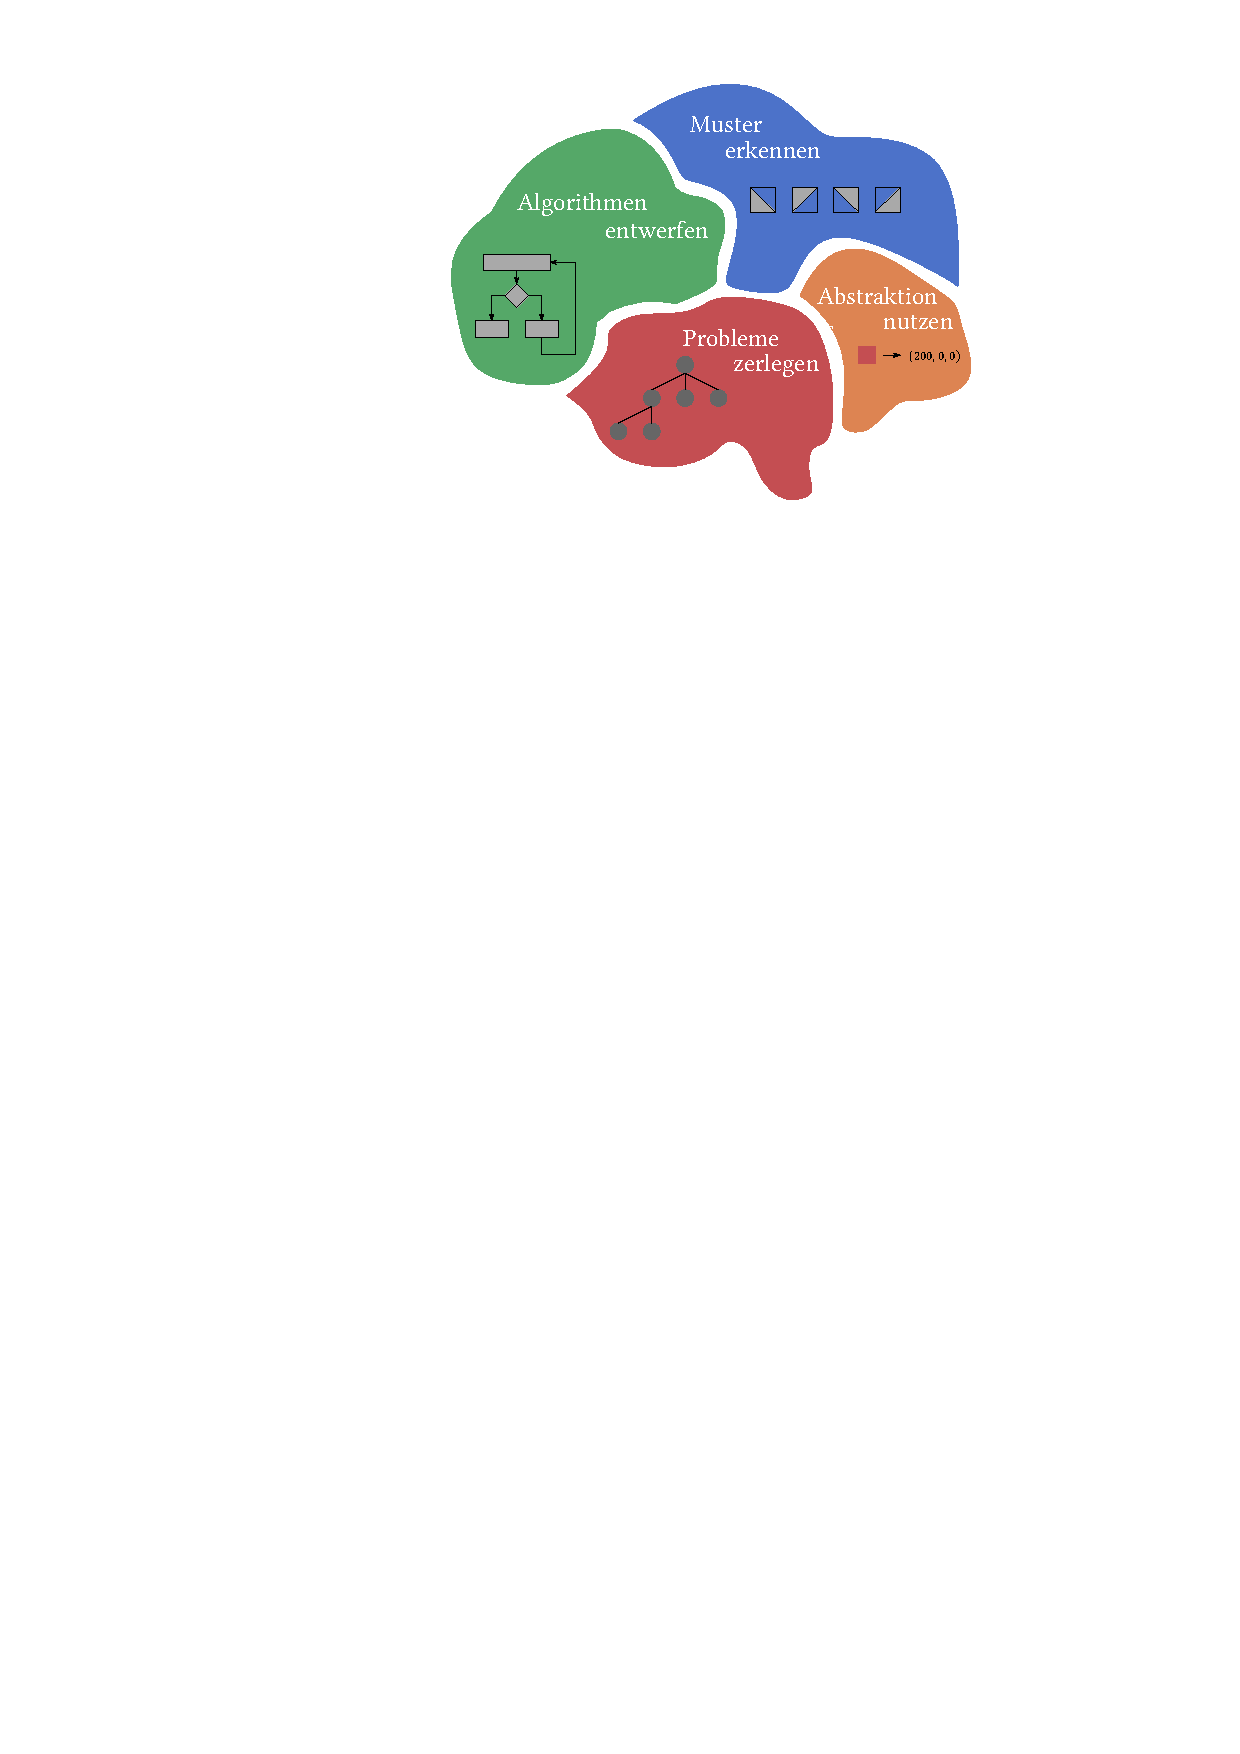
\includegraphics[scale=0.5]{./figs/ct-logo}
	\end{center}
\end{frame}

\begin{frame}
	\frametitle{Was verstehen wir unter CT?}
	Computational Thinking
	\begin{enumerate}[label=$\bullet$]
		\item ist eine Aktivität
		\item bedeutet primär konzipieren (Programmierung als Mittel)
		\item ist eine fundamentale Fähigkeit
		\item ist eine Denkweise des Menschen (nicht der Maschine)
		\item kombiniert analytisches, abstraktes und schaffendes Denken
	\end{enumerate}
\end{frame}

\begin{frame}
	\frametitle{Warum CT?}
	Drei wesentliche Punkte weshalb wir CT für so wichtig halten sind:
	\begin{enumerate}[label=(\arabic*)]
		\item Intrinsischer Wert
		\item (Langfristiger) Nutzen
		\item Selbstbestimmung in der digitalen Ära
	\end{enumerate}
\end{frame}

\begin{frame}
	\frametitle{Lerninhalte}
	Die Auswahl der Lerninhalte viel uns schwer und steht offen zur Diskussion.
	\begin{enumerate}[label=(\arabic*)]
		\item Informationsverarbeitung des digitalen Computers: 
		\begin{enumerate}[label=$\bullet$]
			\item Interpretation
			\item Repräsentation
			\item Manipulation
			\item $\ldots$
		\end{enumerate}
		\item Datenstrukturen und Algorithmen mit Python
			\begin{enumerate}[label=$\bullet$]
			\item Variablen, Ausdrücke und Funktionsaufrufe
			\item Datentypen (Zahlen, Zeichenketten, Listen, Mengen, Wörterbücher, $\ldots$)
			\item Funktionen
			\item Kontrollstrukturen
			\item OOP
		\end{enumerate}
		\item CT in Aktion
	\end{enumerate}
\end{frame}

\begin{frame}
	\frametitle{Kurskonzept}
	\begin{block}{Rahmen}
		CT besteht aus Vorlesungen (2 SWS) und Praktika (2 SWS).
	\end{block}
	\begin{block}{Ziel}
		\begin{enumerate}[label = $\bullet$]
			\item Lernen durch selbständiges (Wieder-)Entdecken.
			\item Früh ins ``Doing'' kommen
		\end{enumerate}
	 $\Rightarrow$ \textbf{Praktika greifen voraus!}
	\end{block}
	\begin{block}{Bedingungen}
		\begin{enumerate}[label = $\bullet$]
			\item Minimale technische Hürden
			\item ``Intuitive'' und gut dokumentierte Programmiersprache als Werkzeug
			\item Kontinuierliches Feedback beim ``Doing''
			\item Entgegenwirken des ``Nerdfaktors''
		\end{enumerate}
	\end{block}
\end{frame}

\begin{frame}
	\frametitle{Hilfsmittel}
	%Technologien:
	\begin{enumerate}[label = $\bullet$]
		\item Material zum Anfassen: Karten, Bücherstapel, Lampen, $\ldots$
		\item Programmiersprachen: Python (+ JavaScript für \textit{Informatik und Design})
		\item Aufgabengenerierung: \href{https://otter-grader.readthedocs.io/en/latest/}{Otter-Grader}
		\item Entwicklungsumgebung: 
		\begin{enumerate}[label = $\bullet$]
			\item \href{https://jupyter.org/}{Jupyter-Notebooks} (+ \href{https://p5js.org/get-started/}{P5.js sketch})
			\item im JupyterLab oder \href{https://code.visualstudio.com/}{VSCode}
			\item gehostet via \href{https://jupyter.org/hub}{JupyterHub}
		\end{enumerate}
		\item Lehrbuch: \href{https://bzoennchen.github.io/ct-book/intro.html}{Interaktives CT-Buch} als \href{https://jupyterbook.org/en/stable/intro.html}{JupyterBook}
		\item \href{https://robo-world-doc.readthedocs.io/en/latest/index.html}{Roboworld Python Package}
	\end{enumerate}
\end{frame}

\begin{frame}
	\frametitle{Infrastruktur}
	Eigener JupyterHub auf einem Kubernetes-Cluster:
	\begin{figure}
		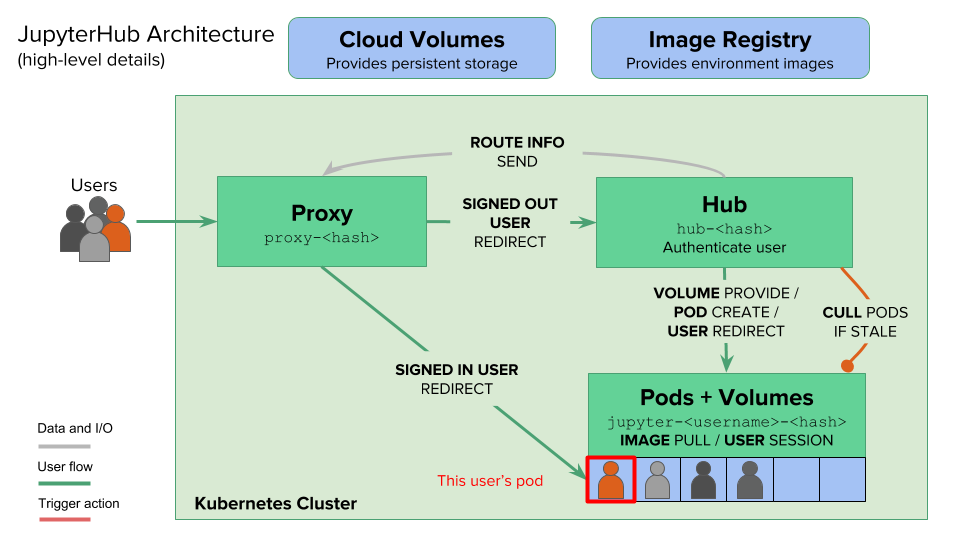
\includegraphics[width=0.75\textwidth]{./figs/infrastructure}
		\caption{Quelle: \href{https://zero-to-jupyterhub.readthedocs.io/en/latest/administrator/architecture.html}{The JupyterHub Architecture}}
	\end{figure}
\end{frame}

\begin{frame}
	\frametitle{Infrastruktur}
	GitLab gespiegelt auf GitHub
\end{frame}

\end{document}
